\documentclass[11pt,a4paper]{article}

% -----------------------------------------------------------------------------
% Paquetes: todos forman parte de una instalacion estandar de LaTeX.
% -----------------------------------------------------------------------------
\usepackage[utf8]{inputenc}
\usepackage{enumitem}
\usepackage{amsmath}
\usepackage{amssymb}
\usepackage{booktabs}
\usepackage[T1]{fontenc}
\usepackage{graphicx}
% Fecha en espanol sin depender de babel ni de spanish.ldf.
\newcommand{\FechaEnEspanol}{%
  \number\day\space de\space
  \ifcase\month
    \or enero\or febrero\or marzo\or abril\or mayo\or junio\or
    julio\or agosto\or septiembre\or octubre\or noviembre\or diciembre
  \fi\space de\space\number\year
}
\usepackage[a4paper,margin=2.5cm,headheight=42pt]{geometry}
\usepackage{graphicx}
\usepackage{xcolor}
\usepackage{fancyhdr}

% lastpage no es necesario para compilar, pero permite mostrar "pagina de N".
\newif\ifHayUltimaPagina
\IfFileExists{lastpage.sty}{
  \usepackage{lastpage}
  \HayUltimaPaginatrue
}{
  \HayUltimaPaginafalse
}

% -----------------------------------------------------------------------------
% CONFIGURACION DEL TRABAJO: editar solamente este bloque para reutilizarlo.
% -----------------------------------------------------------------------------
\newcommand{\NombreMateria}{Redes de Computadoras}
\newcommand{\TipoTrabajo}{Trabajo Práctico}
\newcommand{\NumeroTrabajo}{7}
% Cambiar por "Teórico" o "Práctico" según corresponda.
\newcommand{\TipoTP}{Práctico}
\newcommand{\NombreTrabajo}{Desafío final: captura, de-codificación y recuperación de datos en redes de computadoras}
\newcommand{\NombreGrupo}{NetRunners}
\newcommand{\Docente}{SANTIAGO MARTIN HENN}
\newcommand{\LogoArchivo}{logo.png}
\newcommand{\LogoRuta}{\LogoArchivo}

% Una linea por integrante. Se pueden agregar o quitar filas.
\newcommand{\Integrantes}{%
  \begin{tabular}{ll}
    Bastida, Lucas Ramiro & DNI 39444511 \\
    Contessi, Ruben Andres & DNI 33315235 \\
    Garay, Ignacio Hernan & DNI 44191925 \\
    Giraudo, Juan Pablo & DNI 34970089 \\
    Peñaloza, Gonzalo Adrian & DNI 40441355 \\
    Quinteros del Castillo, Tomás Agustín & DNI 46169739 \\
    Vasconsellos Blason, Benjamin Alejandro & DNI 45642879 \\
  \end{tabular}%
}

% -----------------------------------------------------------------------------
% Elementos comunes de caratula y encabezado.
% -----------------------------------------------------------------------------
\newcommand{\InsertarLogo}[1][0.24\textwidth]{%
  \ifx\LogoRuta\empty
    \fbox{\parbox[c][1cm][c]{#1}{\centering Logo institucional\\\small (colocar archivo)}}%
  \else
    \includegraphics[width=#1,keepaspectratio]{\LogoRuta}%
  \fi
}

\newcommand{\TituloCorto}{TP \NumeroTrabajo (\TipoTP): \NombreTrabajo}

\pagestyle{fancy}
\fancyhf{}
\fancyhead[L]{\InsertarLogo[1.4cm]}
\fancyhead[C]{\small\textbf{\TituloCorto}}
\fancyhead[R]{\small\NombreGrupo}
\renewcommand{\headrulewidth}{0.4pt}
\fancyfoot[C]{\small Pagina \thepage\ifHayUltimaPagina\ de \pageref{LastPage}\fi}
\renewcommand{\footrulewidth}{0pt}

\begin{document}

\begin{titlepage}
  \thispagestyle{empty}
  \begin{center}
    \InsertarLogo[0.32\textwidth]

    \vfill
    {\Large\textsc{\NombreMateria}\par}
    \vspace{1.5cm}
    {\Huge\bfseries \TipoTrabajo\par}
    \vspace{0.35cm}
    {\LARGE N.\textsuperscript{o} \NumeroTrabajo (\TipoTP)\par}
    \vspace{0.8cm}
    {\Large\NombreTrabajo\par}

    \vfill
    \begin{tabular}{rl}
      \textbf{Grupo:} & \NombreGrupo \\
      \textbf{Docente:} & \Docente
    \end{tabular}

    \vspace{1cm}
    \begin{center}
      \textbf{Integrantes}\\[0.2cm]
      \Integrantes
    \end{center}

    \vfill
    {\large \FechaEnEspanol\par}
  \end{center}
\end{titlepage}

\subsection*{Ejercicio 1}

\textit{Averigüen su IP y su máscara (\texttt{ipconfig} / \texttt{ip addr}) y calculen la dirección de broadcast de la red. ¿Cuál es la dirección MAC de broadcast?}

\medskip

Conectados a la red Wi-Fi de la cátedra por DHCP, ejecutamos \texttt{ipconfig} en Windows. El dato relevante es el del adaptador de LAN inalámbrica Wi-Fi:

\begin{center}
\begin{tabular}{|l|l|}
\hline
\textbf{Dato} & \textbf{Valor} \\
\hline
Dirección IPv4 & 192.168.8.182 \\
Máscara de subred & 255.255.255.0 (/24) \\
Puerta de enlace & 192.168.8.1 \\
\hline
\end{tabular}
\end{center}

El adaptador ``Ethernet 3'' (192.168.56.1) es una interfaz virtual de la PC y no participa de la red del aula.

\paragraph{Cálculo de la dirección de broadcast.} La máscara /24 indica que los primeros 24 bits son de red y los últimos 8 son de host:

\begin{center}
\begin{tabular}{|l|l|l|}
\hline
 & \textbf{Decimal} & \textbf{Binario} \\
\hline
IP & 192.168.8.182 & \texttt{11000000.10101000.00001000.10110110} \\
Máscara & 255.255.255.0 & \texttt{11111111.11111111.11111111.00000000} \\
Red (IP AND máscara) & 192.168.8.0 & \texttt{11000000.10101000.00001000.00000000} \\
Broadcast (bits de host en 1) & 192.168.8.255 & \texttt{11000000.10101000.00001000.11111111} \\
\hline
\end{tabular}
\end{center}

\begin{itemize}
  \item \textbf{Dirección de red:} 192.168.8.0
  \item \textbf{Dirección de broadcast:} 192.168.8.255. Coincide con la IP destino de los paquetes del transmisor, lo que confirma la máscara.
  \item \textbf{Rango de hosts utilizables:} 192.168.8.1 a 192.168.8.254
  \item \textbf{Dirección MAC de broadcast:} \texttt{ff:ff:ff:ff:ff:ff}, los 48 bits en 1. Todas las placas de la red local aceptan las tramas dirigidas a esa dirección.
\end{itemize}

\subsection*{Ejercicio 2}

\textit{Abran Wireshark en la interfaz Wi-Fi y capturen al menos 2 minutos. Pueden llegar varios mensajes; no tienen por qué ser todos idénticos.}

\medskip

Capturamos en la interfaz Wi-Fi durante más de dos minutos. Para aislar los mensajes del transmisor usamos el filtro \texttt{frame contains "SIZE"}, ya que la consigna adelantaba que la carga era un JSON con ese campo. También sirve \texttt{eth.dst == ff:ff:ff:ff:ff:ff \&\& udp}, que muestra todo el tráfico de difusión. La captura se guardó en formato \texttt{.pcapng} y se entrega junto con el informe.

\begin{figure}[h]
  \centering
  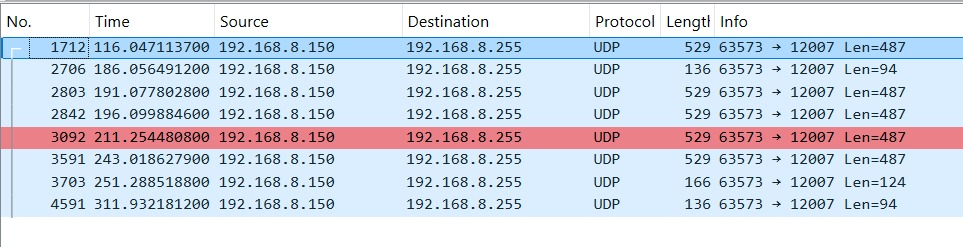
\includegraphics[width=\textwidth]{ejercicio2.jpeg}
  \caption{Datagramas UDP del transmisor capturados en Wireshark.}
  \label{fig:ejercicio2}
\end{figure}

En la primera captura (de los 116\,s a los 312\,s) llegaron 8 datagramas del transmisor, todos de 192.168.8.150:63573 a 192.168.8.255:12007, con tres tamaños de carga distintos (Figura~\ref{fig:ejercicio2}):

\begin{center}
\begin{tabular}{|c|l|l|}
\hline
\textbf{Carga} & \textbf{Tramas} & \textbf{Contenido} \\
\hline
487 bytes & 1712, 2803, 2842, 3092, 3591 & Mensaje 1 (SIZE 8,7), repetido aprox.\ cada 30\,s \\
94 bytes & 2706, 4591 & [Completar] \\
124 bytes & 3703 & [Completar] \\
\hline
\end{tabular}
\end{center}

Detalle del primer mensaje (trama 1712):

\begin{center}
\begin{tabular}{|l|l|l|}
\hline
\textbf{Capa} & \textbf{Campo} & \textbf{Valor} \\
\hline
Trama & Tamaño & 529 bytes (4232 bits) \\
Ethernet II & MAC origen & \texttt{dc:90:09:ed:91:35} (Intel) \\
Ethernet II & MAC destino & \texttt{ff:ff:ff:ff:ff:ff} (broadcast) \\
IPv4 & IP origen & 192.168.8.150 \\
IPv4 & IP destino & 192.168.8.255 (broadcast de la red) \\
UDP & Puerto origen / destino & 63573 / 12007 \\
Datos & Carga útil & 487 bytes de texto ASCII \\
\hline
\end{tabular}
\end{center}

Los tamaños cierran: 14 bytes de Ethernet + 20 de IPv4 + 8 de UDP + 487 de datos = 529 bytes. Que el transporte sea UDP tiene sentido, porque TCP no puede hacer broadcast: una conexión TCP siempre es entre dos extremos.

Para extraer la carga útil hicimos clic derecho sobre la capa \textit{Data} $\rightarrow$ \textit{Copiar} $\rightarrow$ \textit{\ldots as ASCII Text}.

Más tarde el transmisor envió una segunda tanda con otros dos mensajes válidos (mensajes 2 y 3), que también capturamos. Consideramos válido un paquete que trae los campos SIZE, PL y CHECK y cuyos largos cierran con SIZE (ver punto 3); los demás los descartamos. En total analizamos \textbf{tres mensajes válidos distintos}:

\begin{center}
\begin{tabular}{|c|c|c|c|c|}
\hline
\textbf{Mensaje} & \textbf{SIZE} & \textbf{Largo de PL} & \textbf{Largo de CHECK} & \textbf{Datos del JSON} \\
\hline
1 & 8,7 & 392 & 57 & 487 bytes \\
2 & 10,6 & 420 & 52 & 511 bytes \\
3 & 4,4 & 112 & 32 & 182 bytes \\
\hline
\end{tabular}
\end{center}

\subsection*{Ejercicio 3}

\textit{Analicen la estructura del mensaje. ¿Qué formato tiene? ¿Qué campos contiene y qué creen que representa cada uno? Con lo visto en la sección 1, propongan cómo hay que interpretar los datos.}

\medskip

La carga útil es un objeto \textbf{JSON} con tres campos de texto:

\begin{verbatim}
{"SIZE": "8,7", "PL": "110100011101...", "CHECK": "011111010110..."}
\end{verbatim}

\begin{center}
\begin{tabular}{|l|p{11cm}|}
\hline
\textbf{Campo} & \textbf{Qué representa} \\
\hline
SIZE & Tamaño de la matriz, en formato FILAS,COLUMNAS. Las columnas se cuentan en \textbf{caracteres}. \\
PL & La carga (\textit{payload}): los bits de datos, fila por fila. \\
CHECK & Los bits de control: primero la paridad par de cada fila (de arriba hacia abajo) y después la de cada columna (de izquierda a derecha). \\
\hline
\end{tabular}
\end{center}

Interpretación propuesta, según la sección 1:

\begin{enumerate}
  \item Cada carácter ocupa 7 bits ASCII, así que una fila de $C$ caracteres tiene $7C$ bits. Con SIZE ``8,7'' quedan 8 filas de 7 caracteres, o sea 8 filas de 49 bits.
  \item El largo de PL tiene que ser $\mbox{filas} \times 7 \times \mbox{columnas}$: $8 \times 49 = 392$ bits.
  \item El largo de CHECK tiene que ser $\mbox{filas} + 7 \times \mbox{columnas}$: $8 + 49 = 57$ bits (8 de paridad de filas y 49 de columnas).
  \item Se corta PL en filas, se recalcula la paridad par de cada fila y de cada columna, y se compara con CHECK. Las filas y columnas que no coinciden forman el síndrome.
  \item Después de corregir, cada fila se decodifica de a 7 bits con \texttt{decodificar\_mensaje.py}.
\end{enumerate}

Los tres mensajes cumplen estas reglas: $392 = 8 \times 49$ y $57 = 8 + 49$; $420 = 10 \times 42$ y $52 = 10 + 42$; $112 = 4 \times 28$ y $32 = 4 + 28$.

Un detalle: los unos y ceros viajan como caracteres ASCII (``1'' y ``0'', un byte cada uno), no como bits reales. Es solo por el valor didáctico del laboratorio; un código de detección y corrección de errores real opera directamente sobre los bits.

\subsection*{Ejercicio 4}

\textit{Verifiquen la integridad del mensaje con el código de la sección 1: recalculen las paridades y compárenlas con las recibidas. Registren qué filas y qué columnas fallan (el síndrome).}

\medskip

\noindent\textbf{Procedimiento:}
\begin{enumerate}
  \item Para cada mensaje cortamos PL en filas según SIZE (7 bits por carácter).
  \item Calculamos la paridad par de cada fila y de cada columna con \texttt{paridad.py}.
  \item Comparamos el resultado con CHECK. Sus primeros bits son las paridades de las filas, de arriba hacia abajo, y el resto las de las columnas, de izquierda a derecha.
\end{enumerate}

Las filas y columnas donde no coinciden forman el \textbf{síndrome}. En las comparaciones de columnas, las paridades van agrupadas de a 7 (un carácter por grupo) y \texttt{\^{}} marca cada columna que falla.

\subsubsection*{Mensaje 1 (SIZE 8,7: 8 filas de 49 bits; CHECK = 8 + 49 bits)}

\begin{center}
\begin{tabular}{|c|c|c|c|}
\hline
\textbf{Fila} & \textbf{Calculada} & \textbf{Recibida} & \textbf{Resultado} \\
\hline
1 & 0 & 0 & OK \\
2 & 1 & 1 & OK \\
3 & 1 & 1 & OK \\
4 & 1 & 1 & OK \\
5 & 0 & 1 & \textbf{Falla} \\
6 & 0 & 1 & \textbf{Falla} \\
7 & 1 & 0 & \textbf{Falla} \\
8 & 1 & 1 & OK \\
\hline
\end{tabular}
\end{center}

\begin{verbatim}
Columnas calculadas: 0110111 1011101 1011110 0001111 0011000 0110011 0010001
Columnas recibidas:  0110111 1111101 1001110 0101111 0011000 0110011 0010001
                     ....... .^..... ..^.... .^..... ....... ....... .......
\end{verbatim}

\noindent\textbf{Síndrome:} filas 5, 6 y 7; columnas 9, 17 y 23.

\subsubsection*{Mensaje 2 (SIZE 10,6: 10 filas de 42 bits; CHECK = 10 + 42 bits)}

\begin{center}
\begin{tabular}{|c|c|c|c|}
\hline
\textbf{Fila} & \textbf{Calculada} & \textbf{Recibida} & \textbf{Resultado} \\
\hline
1 & 0 & 1 & \textbf{Falla} \\
2 & 0 & 0 & OK \\
3 & 0 & 0 & OK \\
4 & 0 & 0 & OK \\
5 & 1 & 0 & \textbf{Falla} \\
6 & 1 & 0 & \textbf{Falla} \\
7 & 0 & 0 & OK \\
8 & 0 & 1 & \textbf{Falla} \\
9 & 0 & 0 & OK \\
10 & 0 & 0 & OK \\
\hline
\end{tabular}
\end{center}

\begin{verbatim}
Columnas calculadas: 1000011 1110100 1010110 1110001 1010100 1011001
Columnas recibidas:  1010011 1110000 1011110 1111001 1010100 1011001
                     ..^.... ....^.. ...^... ...^... ....... .......
\end{verbatim}

\noindent\textbf{Síndrome:} filas 1, 5, 6 y 8; columnas 3, 12, 18 y 25.

\subsubsection*{Mensaje 3 (SIZE 4,4: 4 filas de 28 bits; CHECK = 4 + 28 bits)}

\begin{center}
\begin{tabular}{|c|c|c|c|}
\hline
\textbf{Fila} & \textbf{Calculada} & \textbf{Recibida} & \textbf{Resultado} \\
\hline
1 & 0 & 1 & \textbf{Falla} \\
2 & 1 & 0 & \textbf{Falla} \\
3 & 1 & 0 & \textbf{Falla} \\
4 & 1 & 0 & \textbf{Falla} \\
\hline
\end{tabular}
\end{center}

\begin{verbatim}
Columnas calculadas: 1110101 0110010 0000101 0100000
Columnas recibidas:  1110100 0111010 1000111 0100000
                     ......^ ...^... ^....^. .......
\end{verbatim}

\noindent\textbf{Síndrome:} las 4 filas; columnas 7, 11, 15 y 20.

\paragraph{Conclusión.} Ningún mensaje llegó intacto. En los tres, la cantidad de filas que fallan es igual a la de columnas que fallan (3 y 3, 4 y 4, 4 y 4), y no hay filas sin columna ni columnas sin fila. Eso indica errores en bits de datos, uno por fila y cada uno en una columna distinta, y no en los bits de control: un bit de control dañado haría fallar una sola fila o una sola columna, sin su pareja. Como hay más de un error por mensaje, el síndrome dice qué filas y columnas están afectadas, pero no cómo se emparejan. Eso se resuelve en el punto 5.

\subsection*{Ejercicio 5}

\textit{Si hay errores, ubíquenlos y corríjanlos. Para cada bit corregido indiquen fila, columna, valor recibido y valor corregido. Si recibieron más de un mensaje distinto, analicen cada uno por separado.}

\medskip

Los tres mensajes tenían \textbf{más de un error}, uno por fila y cada uno en una columna distinta. Con un solo error, el bit dañado estaría en el cruce de la única fila y la única columna que fallan. Con varios errores, la paridad dice qué filas y qué columnas fallan, pero no qué columna va con cada fila. Con $k$ errores hay $k!$ formas de emparejarlas (6 con 3 errores, 24 con 4) y \textbf{todas dejan la paridad consistente}, porque cada una invierte exactamente un bit en cada fila y cada columna que falla. Para elegir, decodificamos cada candidato y nos quedamos con la única combinación que da un texto válido.

Para ubicar el carácter afectado: la columna $c$ corresponde al carácter $\lceil c/7 \rceil$ de la fila, en su bit $(c-1) \bmod 7 + 1$.

\subsubsection*{Mensaje 1 (SIZE 8,7)}

Síndrome: filas 5, 6 y 7; columnas 9, 17 y 23.

Sin corregir se leía \texttt{https://youtube.com/shorts/q8wgKzJwPa\$?featurE=share}:
\begin{itemize}
  \item En la fila 7, solo la columna 23 arregla la palabra (``featurE'' $\rightarrow$ ``feature'').
  \item En la fila 6, la columna 23 da un carácter no imprimible y la columna 9 deja el \texttt{\$}, que no es válido en una URL; solo la columna 17 lo convierte en ``4''.
  \item A la fila 5 le queda la columna 9.
\end{itemize}

\begin{center}
\begin{tabular}{|c|c|c|c|l|}
\hline
\textbf{Fila} & \textbf{Columna} & \textbf{Recibido} & \textbf{Corregido} & \textbf{Carácter} \\
\hline
5 & 9 & 1 & 0 & \texttt{1110111} (w) $\rightarrow$ \texttt{1010111} (W) \\
6 & 17 & 0 & 1 & \texttt{0100100} (\$) $\rightarrow$ \texttt{0110100} (4) \\
7 & 23 & 0 & 1 & \texttt{1000101} (E) $\rightarrow$ \texttt{1100101} (e) \\
\hline
\end{tabular}
\end{center}

\subsubsection*{Mensaje 2 (SIZE 10,6)}

Síndrome: filas 1, 5, 6 y 8; columnas 3, 12, 18 y 25.

Sin corregir: \texttt{xttps://youtube.com/shortw/WCi5h\}1EqqI?featurm=share}:
\begin{itemize}
  \item La fila 1 solo se arregla con la columna 3 (``xttps'' $\rightarrow$ ``https'').
  \item La fila 8, con la columna 25 (``featurm'' $\rightarrow$ ``feature'').
  \item La fila 5, con la columna 12 (``shortw'' $\rightarrow$ ``shorts'').
  \item A la fila 6 le queda la columna 18, que cambia la \texttt{\}} (inválida en una URL) por ``u''.
\end{itemize}

\begin{center}
\begin{tabular}{|c|c|c|c|l|}
\hline
\textbf{Fila} & \textbf{Columna} & \textbf{Recibido} & \textbf{Corregido} & \textbf{Carácter} \\
\hline
1 & 3 & 1 & 0 & \texttt{1111000} (x) $\rightarrow$ \texttt{1101000} (h) \\
5 & 12 & 1 & 0 & \texttt{1110111} (w) $\rightarrow$ \texttt{1110011} (s) \\
6 & 18 & 1 & 0 & \texttt{1111101} (\}) $\rightarrow$ \texttt{1110101} (u) \\
8 & 25 & 1 & 0 & \texttt{1101101} (m) $\rightarrow$ \texttt{1100101} (e) \\
\hline
\end{tabular}
\end{center}

\subsubsection*{Mensaje 3 (SIZE 4,4)}

Síndrome: las 4 filas; columnas 7, 11, 15 y 20.

Sin corregir: \texttt{Qr3mi8!:)1p-dIgZ}. No es una URL ni una palabra, así que probamos las 24 combinaciones. Casi todas dan texto sin sentido (por ejemplo, \texttt{Qz3mh8!:)10-dIeZ} o \texttt{Pr3mi8a:)9p-dIeZ}). Solo una da un mensaje legible, escrito en \textit{leet} (números en lugar de letras): \textbf{\texttt{Pr3mi0!:)10-dIeZ}}, es decir, ``Premio! :) 10 diez''.

\begin{center}
\begin{tabular}{|c|c|c|c|l|}
\hline
\textbf{Fila} & \textbf{Columna} & \textbf{Recibido} & \textbf{Corregido} & \textbf{Carácter} \\
\hline
1 & 7 & 1 & 0 & \texttt{1010001} (Q) $\rightarrow$ \texttt{1010000} (P) \\
2 & 11 & 1 & 0 & \texttt{0111000} (8) $\rightarrow$ \texttt{0110000} (0) \\
3 & 15 & 1 & 0 & \texttt{1110000} (p) $\rightarrow$ \texttt{0110000} (0) \\
4 & 20 & 1 & 0 & \texttt{1100111} (g) $\rightarrow$ \texttt{1100101} (e) \\
\hline
\end{tabular}
\end{center}

En los tres casos, después de corregir volvimos a correr \texttt{paridad.py} y todas las filas y columnas coinciden con CHECK.

\subsection*{Ejercicio 6}

\textit{Construyan un archivo de texto en el formato de mensaje.txt con los datos ya corregidos y decodifíquenlo con decodificar\_mensaje.py (o el cuaderno). Si todo salió bien, el mensaje les va a indicar cómo seguir. Ojo: un mensaje que ``se lee bien'' no es necesariamente un mensaje correcto.}

\medskip

Con los bits corregidos armamos un archivo por mensaje en el formato de \texttt{mensaje.txt}, con una fila de la matriz por línea. Después los decodificamos con \texttt{python decodificar\_mensaje.py corregidoN.txt}.

\paragraph{Mensaje 1} (\texttt{corregido1.txt}):
\begin{verbatim}
1101000111010011101001110000111001101110100101111
0101111111100111011111110101111010011101011100010
1100101010111011000111101111110110101011111110011
1101000110111111100101110100111001101011111110001
0111000101011111001111001011111101010010101110111
1010000110000101101000111111110011011001011100001
1110100111010111100101100101011110111100111101000
1100001111001011001010100000010000001000000100000
\end{verbatim}
Salida: \texttt{https:/}, \texttt{/youtub}, \texttt{e.com/s}, \texttt{horts/q}, \texttt{8WgKzJw}, \texttt{Pa4?fea}, \texttt{ture=sh}, \texttt{are} (más espacios de relleno). Mensaje: \textbf{\texttt{https://youtube.com/shorts/q8WgKzJwPa4?feature=share}}

\paragraph{Mensaje 2} (\texttt{corregido2.txt}):
\begin{verbatim}
110100011101001110100111000011100110111010
010111101011111111001110111111101011110100
111010111000101100101010111011000111101111
110110101011111110011110100011011111110010
111010011100110101111101011110000111101001
011010111010001110101011000110001011110001
111000110010010111111110011011001011100001
111010011101011110010110010101111011110011
110100011000011110010110010101000000100000
010000001000000100000010000001000000100000
\end{verbatim}
Mensaje: \textbf{\texttt{https://youtube.com/shorts/WCi5hu1EqqI?feature=share}}. La última fila es solo de espacios de relleno.

\paragraph{Mensaje 3} (\texttt{corregido3.txt}):
\begin{verbatim}
1010000111001001100111101101
1101001011000001000010111010
0101001011000101100000101101
1100100100100111001011011010
\end{verbatim}
Mensaje: \textbf{\texttt{Pr3mi0!:)10-dIeZ}} (``Premio! :) 10 diez'').

\section*{Reflexiones e investigación}

\subsection*{Reflexión 1}

\textit{¿Qué hubiera pasado si el mensaje tenía errores en dos bits de filas y columnas distintas? ¿Y si se dañaba un bit de los de control?}

\medskip

\paragraph{Dos errores en filas y columnas distintas.} Supongamos errores en (fila 2, columna 3) y (fila 5, columna 8). Fallan 2 filas (2 y 5) y 2 columnas (3 y 8), lo que deja 4 cruces candidatos: (2,3), (2,8), (5,3) y (5,8). Los dos errores pueden ser $\{(2,3),(5,8)\}$ o $\{(2,8),(5,3)\}$, y cualquiera de los dos pares, al invertirse, deja todas las paridades consistentes. El código \textbf{detecta} que hubo errores pero \textbf{no puede corregirlos} con certeza: hace falta otra información, como el contexto o una retransmisión. Es lo que nos pasó, ampliado, con los 3 y 4 errores de nuestros mensajes (6 y 24 combinaciones posibles).

Hay dos variantes peores:
\begin{itemize}
  \item \textbf{Dos errores en la misma fila:} esa fila no aparece en el síndrome (sus dos cambios se cancelan) y solo fallan dos columnas, así que no se sabe en qué fila están.
  \item \textbf{Cuatro errores en las esquinas de un rectángulo:} se cancelan en todas las filas y columnas y no se detectan.
\end{itemize}

\paragraph{Un bit de control dañado.} Falla solo una fila (si era una paridad de fila) o solo una columna (si era de columna), sin su pareja. Esa asimetría lo delata: los datos están bien y no hay que corregir nada. En nuestros tres mensajes no pasó, porque siempre fallaron tantas filas como columnas.

\subsection*{Reflexión 2}

\textit{Si el mensaje es texto en castellano, muchas veces un error ``se adivina'' por contexto (Hola mondo). ¿Sirve eso para una contraseña, un número de cuenta o una dirección web? ¿Qué aporta el código frente a ``leer y adivinar''?}

\medskip

No sirve. En un texto en castellano la redundancia del idioma permite adivinar, pero en una contraseña o un número de cuenta cualquier combinación es igual de válida: un dígito cambiado sigue siendo un número posible. En una dirección web el contexto ayuda solo en parte, y lo vimos en el desafío:
\begin{itemize}
  \item Las palabras fijas se adivinaban fácil (``xttps'' $\rightarrow$ ``https'', ``featurm'' $\rightarrow$ ``feature'').
  \item En el ID del video no hay contexto: ``q8wgKzJw'' y ``q8WgKzJw'' son igual de plausibles, y solo uno lleva al video correcto.
  \item El mensaje 3 es el caso extremo. \texttt{Pr3mi0!:)10-dIeZ} tiene forma de contraseña, y si no hubiera estado escrito en leet, ninguna de las 24 combinaciones habría sido ``más legible'' que otra.
\end{itemize}

Además, adivinar tiene un riesgo silencioso: un texto que ``se lee bien'' puede estar mal y nadie se da cuenta.

El código aporta:
\begin{itemize}
  \item \textbf{Detección garantizada:} avisa que hubo un error aunque el texto se lea perfecto.
  \item \textbf{Corrección objetiva:} con un solo error, lo ubica y lo corrige sin ambigüedad.
  \item \textbf{Independencia del contenido:} funciona igual para texto, números, claves o datos binarios.
\end{itemize}

\subsection*{Reflexión 3}

\textit{¿Pudieron confirmar que su corrección es correcta? ¿Cómo?}

\medskip

En parte, y con una salvedad importante. Después de corregir, recalculamos con \texttt{paridad.py} y todas las filas y columnas coinciden con CHECK. Pero con varios errores eso \textbf{no prueba nada}: cualquiera de las $k!$ combinaciones también deja la paridad consistente, porque cada una invierte un bit en cada fila y cada columna afectada. La confirmación vino de otros criterios:

\begin{itemize}
  \item En los tres mensajes era la \textbf{única} combinación que daba un texto válido. Las demás dejaban caracteres imposibles en una URL (\texttt{\$}, \texttt{\}} o caracteres no imprimibles) o texto sin sentido.
  \item Los IDs de YouTube quedaron con 11 caracteres válidos y los links abren un video; un ID mal corregido lleva a un video inexistente.
  \item El mensaje 3 forma una frase coherente.
\end{itemize}

Una confirmación independiente del contenido sería comparar varias copias del mismo mensaje. El transmisor repetía cada mensaje, así que con varias copias con errores en lugares distintos alcanza con quedarse, bit a bit, con el valor que tiene la mayoría (votación por mayoría).

\subsection*{Reflexión 4}

\textit{Investigar y describir con el mayor detalle posible cómo funciona la técnica de corrección Hamming (7,4) y por qué es superior a la demostración didáctica que hicimos en este Laboratorio. Luego, aplicar la técnica sobre la carga útil obtenida en el desafío y elaborar un paquete de datos que podrían transmitir para que, en caso de corrupción, pueda ser recuperado.}

\medskip

\paragraph{Cómo funciona.} Hamming (7,4) toma bloques de 4 bits de datos ($d_1$ a $d_4$) y agrega 3 bits de paridad ($p_1$, $p_2$, $p_3$), formando palabras de 7 bits. Las paridades van en las posiciones que son potencias de 2 (1, 2 y 4). Cada una controla las posiciones cuyo número, escrito en binario, tiene ese bit en 1:

\begin{center}
\begin{tabular}{|l|c|c|c|c|c|c|c|}
\hline
\textbf{Posición} & 1 & 2 & 3 & 4 & 5 & 6 & 7 \\
\hline
\textbf{Binario} & 001 & 010 & 011 & 100 & 101 & 110 & 111 \\
\textbf{Bit} & $p_1$ & $p_2$ & $d_1$ & $p_3$ & $d_2$ & $d_3$ & $d_4$ \\
\hline
\end{tabular}
\end{center}

\begin{itemize}
  \item $p_1 = d_1 \oplus d_2 \oplus d_4$ (cubre las posiciones 1, 3, 5, 7)
  \item $p_2 = d_1 \oplus d_3 \oplus d_4$ (cubre 2, 3, 6, 7)
  \item $p_3 = d_2 \oplus d_3 \oplus d_4$ (cubre 4, 5, 6, 7)
\end{itemize}

Al recibir, el receptor recalcula los tres controles sobre lo que le llegó:
\[
s_1 = b_1 \oplus b_3 \oplus b_5 \oplus b_7, \qquad
s_2 = b_2 \oplus b_3 \oplus b_6 \oplus b_7, \qquad
s_3 = b_4 \oplus b_5 \oplus b_6 \oplus b_7
\]

El número binario $s_3 s_2 s_1$ es el \textbf{síndrome}. Si vale $000$ no hay error; si no, es directamente la \textbf{posición del bit dañado}, y alcanza con invertirlo. Funciona porque cada posición está cubierta por una combinación distinta de paridades, que coincide con su número en binario. La distancia mínima entre palabras válidas es 3: corrige 1 error por bloque, o detecta 2 si no se intenta corregir.

\paragraph{Ejemplo con el carácter ``P''} (ASCII 80 = \texttt{01010000}):
\begin{itemize}
  \item Mitad alta \texttt{0101} ($d_1=0$, $d_2=1$, $d_3=0$, $d_4=1$): $p_1 = 0\oplus1\oplus1 = 0$, $p_2 = 0\oplus0\oplus1 = 1$, $p_3 = 1\oplus0\oplus1 = 0$, así que se transmite \textbf{\texttt{0100101}}.
  \item Mitad baja \texttt{0000}: se transmite \textbf{\texttt{0000000}}.
  \item Si llega \texttt{0100111} (dañada la posición 6): $s_1 = 0\oplus0\oplus1\oplus1 = 0$, $s_2 = 1\oplus0\oplus1\oplus1 = 1$, $s_3 = 0\oplus1\oplus1\oplus1 = 1$. El síndrome $110 = 6$ indica la posición, se invierte ese bit y se recupera \texttt{0101}.
\end{itemize}

\paragraph{Por qué es superior a la paridad bidimensional del laboratorio.}

\begin{center}
\begin{tabular}{|l|p{5.2cm}|p{5.2cm}|}
\hline
 & \textbf{Paridad bidimensional} & \textbf{Hamming (7,4)} \\
\hline
Ubicación del error & Cruce de fila y columna & El síndrome da la posición directamente \\
Errores corregibles & 1 en todo el mensaje & 1 por cada bloque de 7 bits \\
Con 2 o más errores & Ambiguo: hay que adivinar (nos pasó con 3 y 4) & Se corrigen todos si caen en bloques distintos \\
Depende del contenido & Para desempatar, sí & No \\
Redundancia & Baja (filas + columnas) & Alta (3 bits cada 4 de datos) \\
\hline
\end{tabular}
\end{center}

En el mensaje 3, por ejemplo, la paridad 2D agregaba 32 bits de control a 112 de datos. Hamming agrega 96 a 128, pero recupera el mensaje sin ambigüedad.

\paragraph{Aplicación a la carga útil del desafío.} Codificamos el mensaje 3, \texttt{Pr3mi0!:)10-dIeZ} (16 caracteres), con nuestro script \texttt{hamming.py}:
\begin{enumerate}
  \item Cada carácter ASCII se completa a 8 bits.
  \item Se divide en dos mitades de 4 bits.
  \item Cada mitad se codifica en una palabra de 7 bits.
\end{enumerate}
Quedan 14 bits por carácter y 224 bits en total:

\begin{center}
\begin{tabular}{|c|c|c|c|}
\hline
\textbf{Car.} & \textbf{ASCII (8 bits)} & \textbf{Palabra alta} & \textbf{Palabra baja} \\
\hline
P & \texttt{01010000} & \texttt{0100101} & \texttt{0000000} \\
r & \texttt{01110010} & \texttt{0001111} & \texttt{0101010} \\
3 & \texttt{00110011} & \texttt{1000011} & \texttt{1000011} \\
m & \texttt{01101101} & \texttt{1100110} & \texttt{1010101} \\
i & \texttt{01101001} & \texttt{1100110} & \texttt{0011001} \\
0 & \texttt{00110000} & \texttt{1000011} & \texttt{0000000} \\
! & \texttt{00100001} & \texttt{0101010} & \texttt{1101001} \\
: & \texttt{00111010} & \texttt{1000011} & \texttt{1011010} \\
) & \texttt{00101001} & \texttt{0101010} & \texttt{0011001} \\
1 & \texttt{00110001} & \texttt{1000011} & \texttt{1101001} \\
0 & \texttt{00110000} & \texttt{1000011} & \texttt{0000000} \\
- & \texttt{00101101} & \texttt{0101010} & \texttt{1010101} \\
d & \texttt{01100100} & \texttt{1100110} & \texttt{1001100} \\
I & \texttt{01001001} & \texttt{1001100} & \texttt{0011001} \\
e & \texttt{01100101} & \texttt{1100110} & \texttt{0100101} \\
Z & \texttt{01011010} & \texttt{0100101} & \texttt{1011010} \\
\hline
\end{tabular}
\end{center}

El paquete a transmitir, en el mismo estilo JSON que usó la cátedra (archivo \texttt{paquete\_hamming.json}):

\begin{verbatim}
{"CODE": "HAMMING(7,4)", "CHARS": 16, "PL":
 "01001010000000000111101010101000011100001111001101010101
  11001100011001100001100000000101010110100110000111011010
  01010100011001100001111010011000011000000001010101010101
  11001101001100100110000110011100110010010101001011011010"}
\end{verbatim}

\begin{itemize}
  \item \textbf{CODE} indica el código usado.
  \item \textbf{CHARS} indica la cantidad de caracteres, para validar el largo ($16 \times 14 = 224$ bits).
  \item \textbf{PL} son los bits codificados. Acá están partidos en cuatro líneas de 56 bits solo para que entren en la página; en el paquete real van en una sola cadena.
\end{itemize}

\paragraph{Prueba de recuperación.} Invertimos un bit en cuatro bloques distintos (los bits 22, 70, 145 y 176 del paquete) y decodificamos con \texttt{python hamming.py}. El script corrigió los cuatro errores (bloque 4 posición 1, bloque 10 posición 7, bloque 21 posición 5 y bloque 26 posición 1) y recuperó \texttt{Pr3mi0!:)10-dIeZ} sin ambigüedad. Con la paridad bidimensional, esos mismos cuatro errores habrían dejado 24 combinaciones posibles, igual que en el desafío.

\end{document}
